\setlength{\headheight}{14.49998pt}
\addtolength{\topmargin}{-2.49998pt}
\chapter{Contesto di riferimento}\label{ch:Contesto}
La stesura del codice di questo progetto di prova finale è stata effettuata grazie a strumenti digitali basati sul web e ai relativi linguaggi di programmazione. 

L'adozione di una solida architettura informatica ha giocato un ruolo cruciale. 
Prima di descrivere nel dettaglio il contesto client-server utilizzato, è necessario introdurre alcuni concetti fondamentali per la comprensione del progetto.
Questo capitolo esplorerà le piattaforme, i \gls{framework}\footnote{\glsdesc{framework}} e gli strumenti già esistenti \cite{ngrx} \cite{reactivex}, delineando le ragioni dietro la loro scelta e illustrando come si integrano per supportare l'intera struttura dell'applicazione.

\section{Modello three-tier}\label{sec:three-tier}
\begin{figure}[H]
\centering
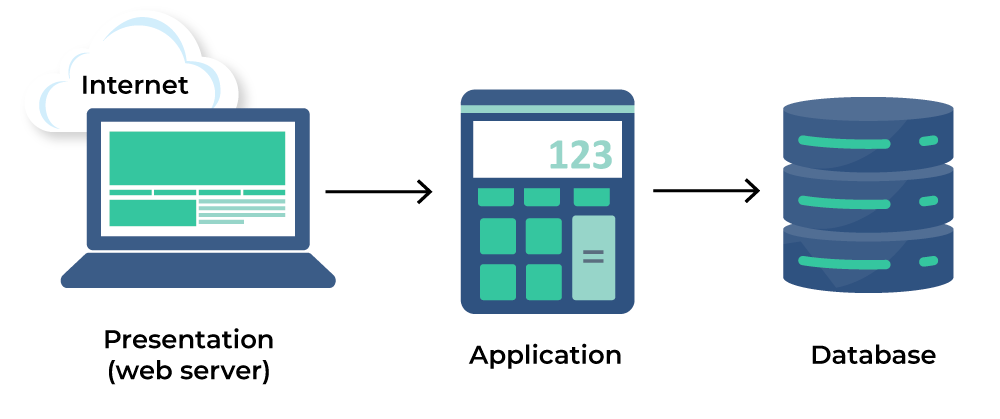
\includegraphics[width=1\textwidth]{Images/3-Tier-architecture.png}
\caption{\label{fig:three-tier}Schema di un'applicazione a tre livelli.}
\end{figure}

Il modello three-tier (a tre livelli) è un'architettura software consolidata, di tipo client-server, in cui l'interfaccia utente, l'elaborazione logica e la gestione dei dati sono sviluppati e mantenuti come moduli indipendenti su server distinti. L'organizzazione in livelli separati aiuta a migliorare lo scopo dell'architettura stessa, aumentando quindi la manutenibilità, la scalabilità, l'affidabilità, la flessibilità e ovviamente la modularità del sistema.

Il maggior beneficio del modello three-tier consiste nel fatto che i livelli sono sviluppati e mantenuti in modo indipendente, con la conseguenza che, in caso di qualsiasi modifica, viene coinvolto solamente il livello modificato. Inoltre, un ulteriore vantaggio è dato dal fatto che i livelli possono essere scalati separatamente, all'aumentare del carico di lavoro di uno qualsiasi.

Come si può intuire dal nome, il modello three-tier è composto da tre livelli: 
\begin{enumerate}
\item livello di presentazione
\item livello di applicazione
\item livello di \acrlong{db}
\end{enumerate}

Nello specifico, il primo livello è quello che viene presentato all'utente finale, ossia l'interfaccia grafica grazie alla quale l'utente ha la possibilità di interagire con il sistema. Lo scopo principale dello strato superiore del modello three-tier è di mostrare le informazioni provenienti dagli altri livelli in modo chiaro e comprensibile all'utente e di raccogliere eventuali dati inseriti dall'utente stesso.
Il livello di presentazione può essere eseguito su un qualsiasi browser web, su un'applicazione desktop o su un'interfaccia grafica (\acrshort{gui}), a seconda delle esigenze del progetto.
Le applicazioni del livello di presentazione, nel caso del web, sono solitamente sviluppate utilizzando HTML, CSS e JavaScript mentre, nel caso delle applicazioni desktop, possono essere scritte in un'ampia varietà di linguaggi a seconda della piattaforma. Recentemente i \gls{framework} per lo sviluppo front-end, come \gls{angular}, React e Vue.js, sono diventati sempre più popolari. In questo progetto di tirocinio è stato scelto il \gls{framework} \gls{angular}, come verrà spiegato più approfonditamente nella sezione \ref{sec:ang+prime}.

Il secondo livello, quello di applicazione (o di logica) raccoglie informazioni e richieste dal livello superiore e le elabora utilizzando le regole specifiche della logica di business. Inoltre, il livello di applicazione può aggiungere, eliminare o modificare i dati memorizzati nel livello di \acrlong{db}. Per esempio, nel caso di un e-commerce, il livello di applicazione fa query\footnote{\glsdesc{query}} al \acrlong{db} dell'inventario per sapere la disponibiltà di un prodotto, oppure aggiunge dettagli al profilo di un cliente, etc.
In breve, è il livello responsabile di processare le richieste del client e, una volta ricevute le informazioni necessarie, di inviarle di nuovo al client.
Nei sistemi più moderni o complessi, questo livello è solitamente sviluppato utilizzando linguaggi come Java, Python, PHP, Ruby, Perl, ASP.NET, \acrlong{js} o \acrlong{ts}, etc. In generale, qualsiasi linguaggio di programmazione che supporti le chiamate \gls{API}\footnote{\glsdesc{API}} (in modo da poter comunicare con il livello del \acrlong{db}, o con altri moduli) può essere utilizzato per sviluppare il livello di applicazione.

Infine, nel terzo livello, detto anche livello di accesso ai dati (\acrlong{db}) o back-end, le informazioni elaborate dall'applicazione vengono archiviate e gestite, in modo da poter essere recuperate in seguito, quando necessario. Il back-end si sostanzia in un \acrfull{dbms} e tra i più diffusi ricordiamo PostgreSQL, MySQL, MariaDB, Oracle, DB2, Informix, Microsoft SQL Server.
\begin{figure}[H]
\centering

\includegraphics[width=.5\textwidth]{Images/Mysql_logo.png}
\caption{\label{fig:mysql}Logo di MySQL.}
\end{figure}

L'architettura a tre livelli viene spesso paragonata all'architettura \acrfull{mvc}:
entrambe cercano di separare le responsabilità e migliorare lo sviluppo del software, ma lo portano a termine diversamente. 

Il modello three-tier si concentra di più sulla separazione dell'applicazione in diversi livelli, specificando una comunicazione ben definita tra di loro, come già discusso in precedenza.

Invece, l'architettura \acrshort{mvc} si concentra di più sulla separazione dell'applicazione all'interno di un livello  in tre componenti distinti: Modello, Vista e Controllore, come si può vedere nella figura \ref{fig:mvc}. Il Modello rappresenta i dati e la logica di business dell'applicazione, la Vista rappresenta l'interfaccia utente e il Controllore agisce come mediatore tra i primi due. Infatti, è il Controllore a ricevere l'input dall'utente, a interagire con il Modello per elaborare i dati e ad aggiornare la Vista per visualizzarne i risultati.

\begin{figure}[H]
\centering
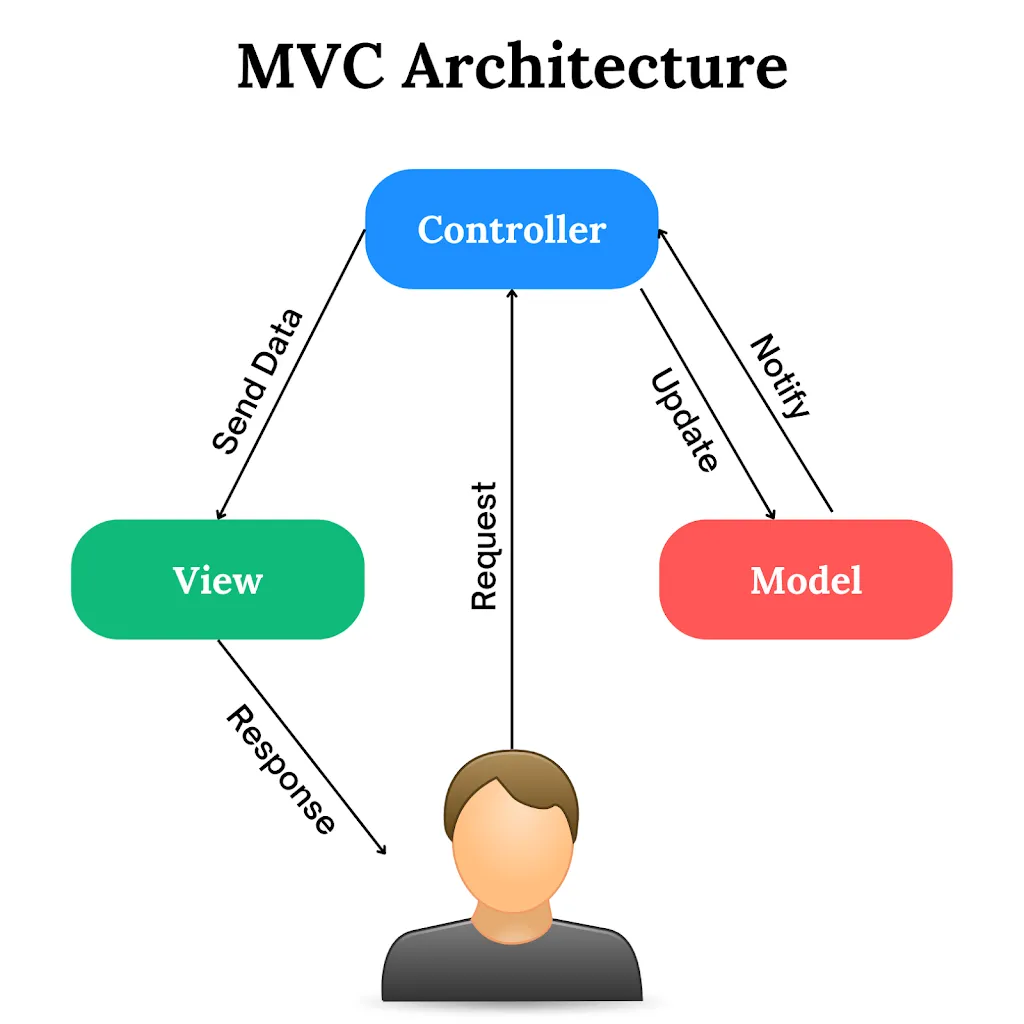
\includegraphics[width=.6\textwidth]{Images/mvc.png}
\caption{\label{fig:mvc}Schema astratto dell'architettura \acrshort{mvc}.}
\end{figure}


 
\section{Framework utilizzati}\label{sec:Framework}
\begin{figure}[H]
\centering
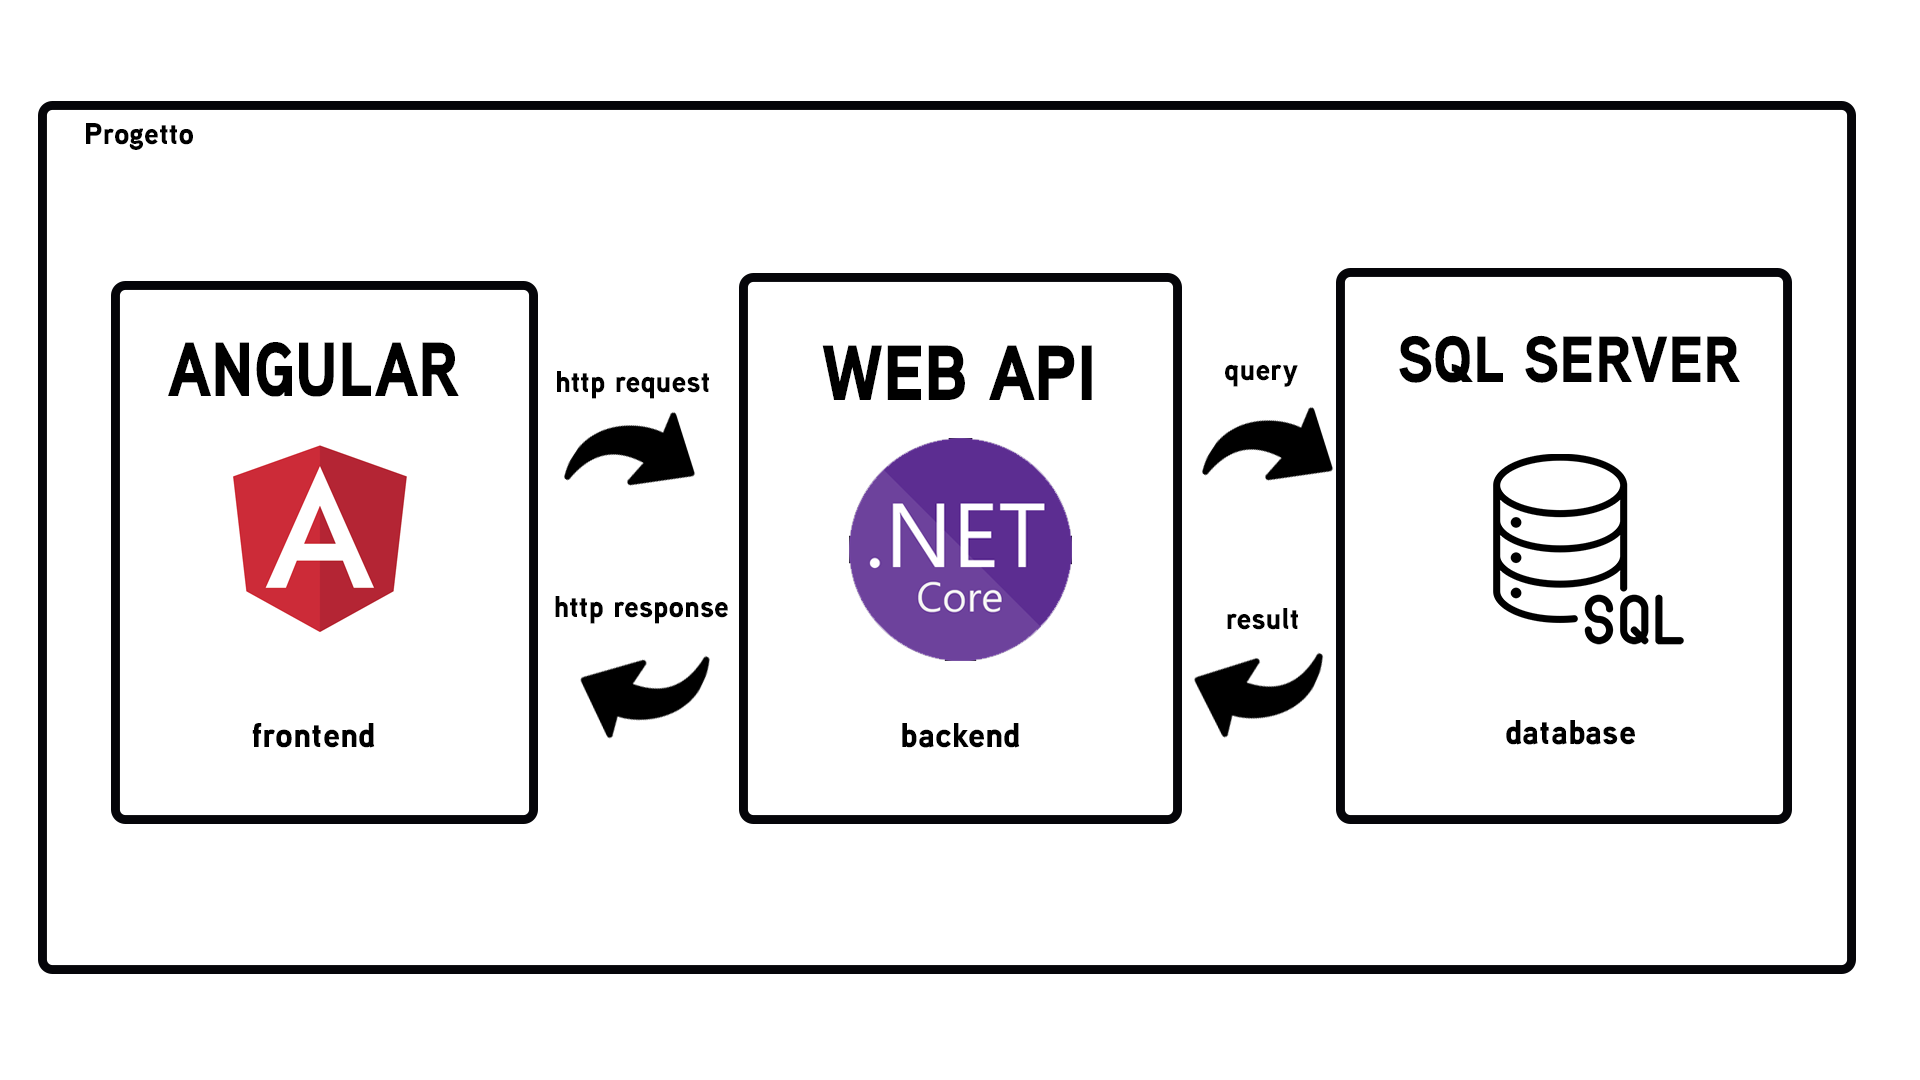
\includegraphics[width=1\textwidth]{Images/architettura.png}
\caption{\label{fig:arch}Schema dei \gls{framework} utilizzati.}
\end{figure}

Un \gls{framework} è un'astrazione che unisce codice comune tra progetti software con scopi simili, fornendo una funzionalità generale, che può essere modificata o estesa per risolvere un problema specifico.
Più in generale, i \gls{framework} per il web, incrementano l'efficienza e le prestazioni dello sviluppo, fornendo una struttura coerente, affinché gli sviluppatori non debbano continuamente scrivere il codice partendo da zero. I \gls{framework} sono quindi ottimi quando si tratta di risparmiare tempo, perchè offrono ai programmatori una serie di funzionalità extra che possono essere aggiunte al software, senza richiedere molto sforzo.

Nel caso di questo progetto di tirocinio, lo scopo principale è stato quello di implementare nuovi componenti e funzionalità per un'applicazione web già esistente, utilizzando i \gls{framework} già adottati nel progetto stesso, senza dover scrivere il codice partendo da zero. Uno dei difetti di questo approccio è stato aver ricevuto del software scritto da più sviluppatori, con stili di programmazione diversi e componenti sviluppati da una o più persone. Infatti la repository dell'intero progetto è composta da più di 55 mila file, con il rischio di perdersi nella moltitudine di elementi.
È stato comunque possibile integrare le nuove funzionalità grazie ai \gls{framework} di sviluppo utilizzati, sia per il back-end che per il front-end.

\subsection{Angular e PrimeNG}\label{sec:ang+prime}
Questa sezione descrive uno dei \gls{framework} per il front-end più utilizzati al mondo, \gls{angular} \cite{angular}, insieme al relativo \gls{framework} \gls{open source}\footnote{\glsdesc{open source}} \acrshort{primeng} \cite{primeng}, che fornisce uno dei set di componenti \acrshort{ui} più completi per \gls{angular}.

\begin{figure}[!htb]
    \centering
    \begin{minipage}{.5\textwidth}
        \centering
        
\includegraphics[width=.5\textwidth]{Images/angular.png}
        \centering
        \caption{\label{fig:ang logo}Logo di Angular.}
    \end{minipage}%
    \begin{minipage}{0.5\textwidth}
        \centering
        
\includegraphics[width=.35\textwidth]{Images/primeng.png}
        \caption{\label{fig:ng logo}Logo di PrimeNG.}
    \end{minipage}
\end{figure}

\gls{angular}, denominato anche \gls{angular} 2+ (ossia una versione più moderna di \gls{angularjs}), è un \gls{framework} \acrlong{js} scritto e basato su \acrlong{ts}, per lo sviluppo delle interfacce delle applicazioni. Sviluppato principalmente dal team \gls{angular} di Google e da una comunità di programmatori e aziende esterne, è una riscrittura completa del \gls{framework} originale (AngularJS). Attualmente, \gls{angular} è mantenuto da Google.

In quanto \gls{framework}, \gls{angular} fornisce una struttura standard per gli sviluppatori. Consente di creare applicazioni di grandi dimensioni, facilmente mantenibili.  

La principale funzionalità di \gls{angular} è quella di fornire blocchi per costruire le applicazioni web, denominati componenti, grazie ai quali gli sviluppatori possono impostare rapidamente applicazioni web scalabili e mantenibili.
I programmatori hanno la libertà di sviluppare applicazioni che possono essere eseguite su più piattaforme, inclusi dispositivi mobili, desktop e web. Essendo progettato per essere modulare, permette di integrare o rimuovere facilmente le funzionalità di cui si ha bisogno o meno.

Alcune caratteristiche \textbf{vantaggiose} di \gls{angular} sono:
\begin{itemize}
    \item \acrlong{dom}: Angular sfrutta il \acrshort{dom} per gestire le pagine web.
    \item \acrfull{ts}: linguaggio, sviluppato da Microsoft, in cui è scritto \gls{angular}. Definisce un insieme di tipi che rende il codice più facile da leggere e da scrivere. Inoltre, tutto il codice \acrlong{ts} viene compilato in \acrlong{js}, cossicché ogni piattaforma possa eseguirlo. \acrlong{ts} è altamente consigliato, ma non vincolante per sviluppare con \gls{angular}.
    \item Data Binding: meccanismo che abilita gli utenti a manipolare gli elementi di una pagina web attraverso un browser web. Usato principalmente nelle pagine web che incorporano componenti interattivi, come calcolatori, tutorial, forum e giochi. Inoltre, consente una migliore visualizzazione progressiva di una pagina web, quando questa contiene una grande quantità di dati. Nel caso di \gls{angular} viene utilizzato un data binding bidirezionale, infatti lo stato del modello riflette eventuali modifiche apportate agli elementi dell'interfaccia corrispondente. Al contrario, lo stato della Vista riflette eventuali modifiche apportate allo stato del Modello e questa funzionalità consente al \gls{framework} di collegare il \acrshort{dom} ai dati del Modello attraverso il Controllore.
    \item Testing: \gls{angular} usa un \gls{framework} denominato Jasmine per il test delle applicazione, ma non sarà oggetto di discussione in questo documento.
\end{itemize}

Passando all'architettura, è importante ricordare che \gls{angular} è un \gls{framework} \acrshort{mvc} a tutti gli effetti e offre una guida chiara su come strutturare applicazioni web.

I blocchi fondamentali di un'applicazione \gls{angular} sono sei, introdotti successivamente:
\begin{enumerate}
    \item Moduli: una web app \gls{angular} possiede un modulo root (denominato AppModule) che fornisce il meccanismo di bootstrap\footnote{\glsdesc{bootstrap}} per avviare l'applicazione. Ogni modulo può avere uno o più moduli figlio.
    \item Componenti: ogni componente dell'applicazione definisce una classe che contiene i dati e la logica dell'applicazione. Generalmente, un componente definisce una parte dell'interfaccia grafica.
    \item Modelli (o Template): contengono il codice della struttura iniziale dell'applicazione, in figura \ref{fig:berry} si può vedere un esempio di template Angular;
    \item Metadati: comunicano ad \gls{angular} come processare e decorare le classi, cosicché si possa configurare il comportamento aspettato della classe.
    \item Servizi: una classe di servizio è creata quando si hanno dati o logica che non sono associati con la visualizzazione, ma devono comunque essere condivisi tra i componenti. La classe di servizio è sempre introdotta con il decoratore `@Injectable'.
    \item Dependency Injection: pattern di progettazione che permette di mantenere le classi dei componenti precise ed efficienti. È una funzionalità che non raccoglie dati da un server, valida un input dell'utente o stampa direttamente a console. Invece, delega i suddetti compiti ai servizi \cite{anginj}.
\end{enumerate}

\begin{figure}[H]
\centering
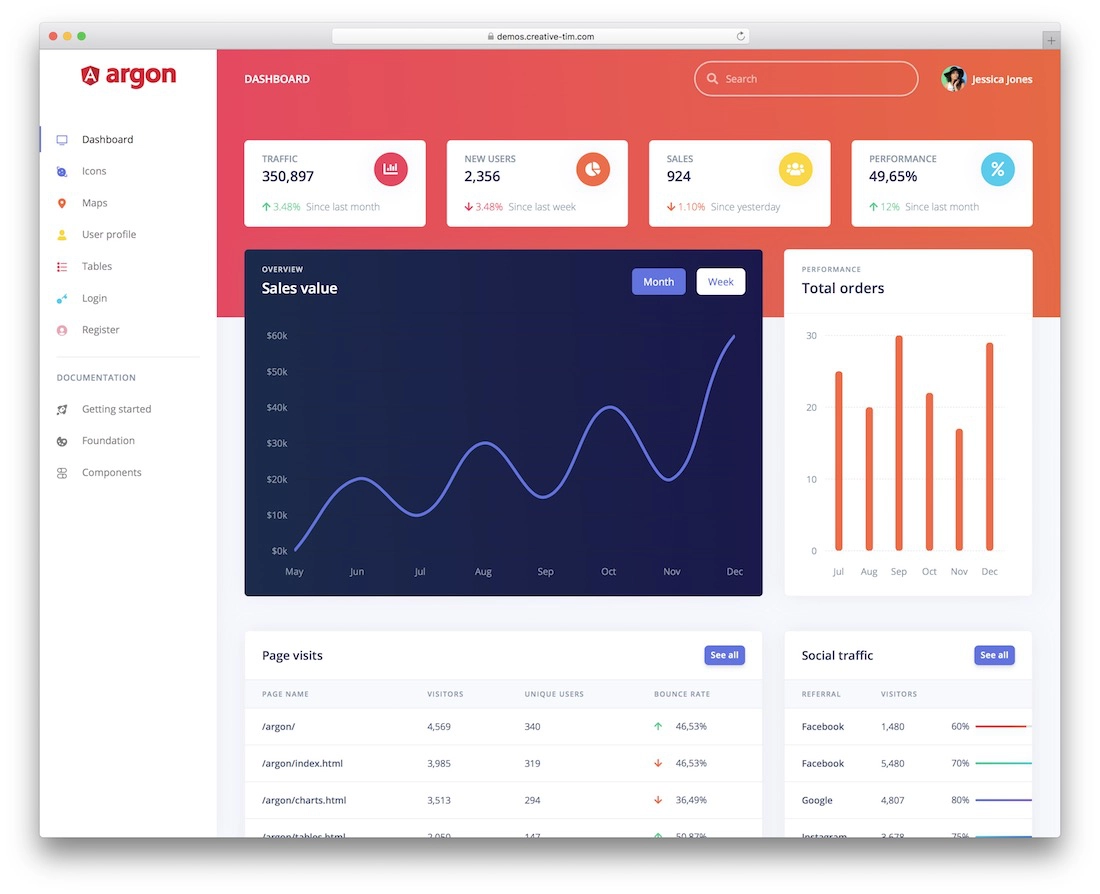
\includegraphics[width=.75\textwidth]{Images/argon.png}
\caption{\label{fig:berry}Argon, un template Angular.}
\end{figure}

Angular ha anche degli \textbf{svantaggi}, tra cui ricordiamo una ripida curva di apprendimento, capacità di Search Engine Optimization limitate, difficoltà nelle migrazioni alle versioni successive e verbosità.

Una ulteriore funzionalità degna di nota di \gls{angular} è la sua \acrfull{cli}, che permette di creare nuovi progetti, applicazioni, componenti, etc. Inoltre, \gls{angular} \acrshort{cli} offre anche la possibilità di eseguire un web server, tramite l'apposito comando da terminale, in modo tale da poter testare l'applicazione in locale, prima di effettuare il \gls{deploy} su un server remoto.
Tra le aziende più famose che utilizzano \gls{angular} ci sono Google, Microsoft, Nike, Forbes, Upwork, HBO, Sony, General Motors, etc.

\begin{figure}[H]
\centering
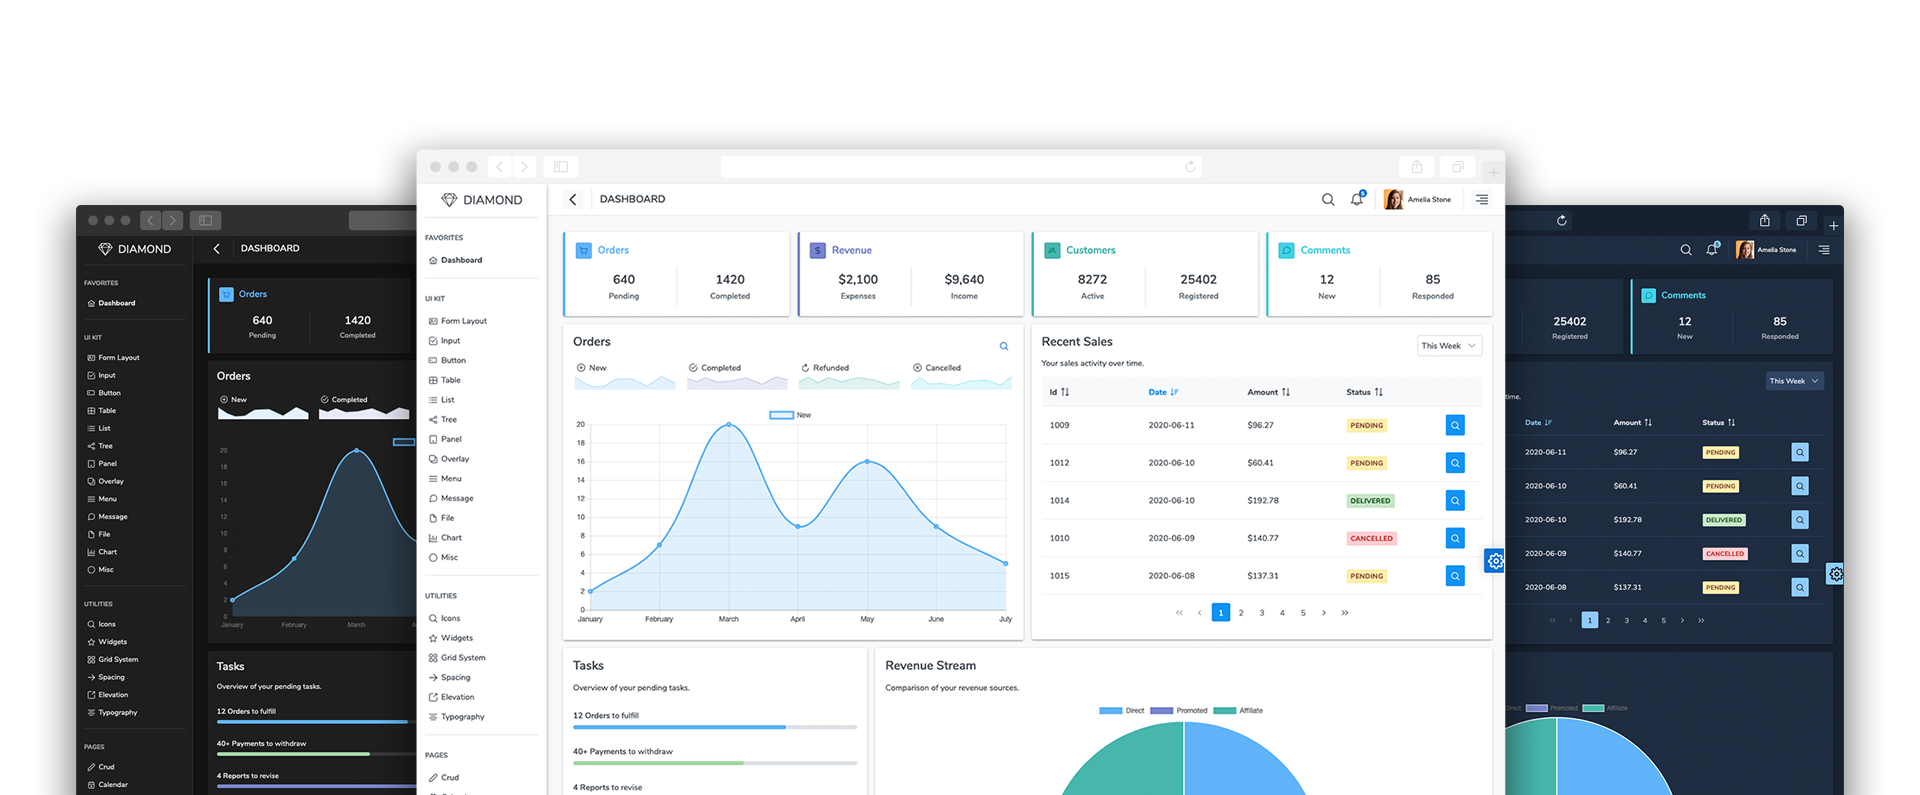
\includegraphics[width=1\textwidth]{Images/diamond.png}
\caption{\label{fig:diamond}Diamond, uno dei template di PrimeNG.}
\end{figure}
% parte di PrimeNG
\acrfull{primeng} è una collezione ricca di componenti \acrshort{ui} per \gls{angular}, i cui widget sono \gls{open source} e gratuiti. Offre oltre 80 componenti \acrshort{ui}, come ad esempio tabelle, grafici, dialoghi, etc.
\acrshort{primeng} supporta inoltre vari temi, permettendo agli sviluppatori di scegliere tra una vasta gamma. La figura \ref{fig:diamond} mostra un esempio di template.

Molte aziende usano \acrshort{primeng} sia per applicazioni interne che per applicazioni per i clienti. Grazie alla sua numerosa serie di componenti e facilità d'uso, \acrshort{primeng} è diventato una delle scelte più popolari e valide tra gli sviluppatori, anche per le applicazioni più complesse. Tra le aziende che usano \acrshort{primeng} troviamo Ericsson, Siemens, Lufthansa, UniCredit, Ford, Volvo, Nvidia, eBay, Mercedes-Benz, Audi, HP, Scania, Cisco, Nike, Wolkswagen.

 
\subsection{Typescript}\label{sec:Typescript}
\begin{figure}[H]
\centering

\includegraphics[width=.7\textwidth]{Images/ts.png}
\caption{\label{fig:logo ts}Logo di TypeScript.}
\end{figure}
\acrfull{ts} \cite{typescript} è un linguaggio di programmazione \gls{open source} sviluppato e mantenuto da Microsoft. È un superset di \acrlong{js}, infatti offre tutte le funzionalità di quest'ultimo, aggiungendone di nuove e più avanzate, come la possibilità di tipare staticamente il linguaggio. Nello specifico, siccome \acrlong{ts} `conosce' il linguaggio \acrlong{js} \cite{articleTS}, in molti casi genererà i tipi inferendoli\footnote{\glsdesc{inferenza}} dal codice. Per esempio, inizializzando una variabile con un valore arbitrario, \acrlong{ts} userà il valore come tipo (Figura \ref{fig:hello}). 

\begin{figure}[H]
\centering
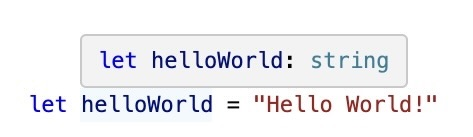
\includegraphics[width=.8\textwidth]{Images/ts hello.jpg}
\caption{\label{fig:hello}Inizializzazione del classico `Helo World!'.}
\end{figure}

Sapendo come funziona \acrlong{js}, \acrlong{ts} può costruire un sistema di tipi che accetta il codice \acrlong{js}. Infatti, è così che \acrlong{ts} è in grado di capire che `helloWorld' è una stringa nell'esempio in figura \ref{fig:hello}.
Visual Studio Code, sviluppato da Microsoft, usa \acrlong{ts} per facilitare l'esperienza della scrittura del codice. 

Inoltre, \acrlong{ts} è stato progettato per lo sviluppo di applicazioni di grandi dimensioni e viene transcompilato\footnote{\glsdesc{transcompilare}} in \acrlong{js}.

Pubblicato nel 2012 da Microsoft, voleva migliorare \acrlong{js} in modo che gli sviluppatori potessero lavorare su applicazioni di grandi dimensioni, cosa difficile con \acrlong{js}. Importanti e numerose sono le funzionalità introdotte da \acrlong{ts}:
\begin{itemize}
    \item Controllo di tipo statico: \acrlong{ts} introduce il controllo di tipo statico, che può rilevare errori a tempo di compilazione, piuttosto che durante l'esecuzione.
    \item Oggetti e classi: una delle caratteristiche principali della programmazione orientata agli oggetti.
    \item Moduli: possono aiutare ad organizzare e incapsulare il codice.
    \item Strumenti avanzati: autocompletamento, navigazione e refactoring\footnote{\glsdesc{refactoring}}.
    \item Scalabilità: grazie a funzionalità quali tipi, classi e moduli, \acrlong{ts} è particolarmente adatto per applicazioni di grandi dimensioni.
\end{itemize}

Tra le aziende più famose che utilizzano \acrlong{ts} ricordiamo Google, Slack, Medium, Doordash, bitpanda e Techstack.


 
\subsection{\text{.NET} Framework, \text{.NET} Core e \text{.NET} 8}\label{sec:.net} 
\begin{figure}[H]
\centering

\includegraphics[width=.7\textwidth]{Images/net.png}
\caption{\label{fig:.net}Logo di \gls{.net} Framework.}
\end{figure}
\gls{.net} \cite{dotnet} è un \gls{framework} \gls{software} sviluppato da Microsoft, che include una vasta libreria di classi, denominata \acrlong{fcl} e fornisce interoperabilità tra diversi linguaggi di programmazione \cite{.net}.
Inizialmente rilasciato nel 2002 \cite{.netHistory}, \gls{.net} nasce come software proprietario, ma negli anni successivi Microsoft ha rilasciato le versioni \gls{open source}.
\gls{.net} \cite{dotnetVideos} è usato da milioni di sviluppatori in tutto il mondo per creare applicazioni per una moltitudine di piattaforme e dispositivi.

Successivamente a \gls{.net} Framework, Microsoft ha rilasciato \gls{.net} Core, una versione più leggera e veloce della precedente, che può essere eseguita su Windows, Linux e macOS, grazie a una nuova architettura modulare e flessibile. Infatti, è possibile scegliere direttamente i componenti di cui si necessita e implementarli subito, senza dover installare il \gls{framework} completo. \gls{.net} ha una vasta comunità di sviluppatori che contribuiscono alla creazione di strumenti, librerie e documentazione, il che rende più semplice per gli sviluppatori ottenere aiuto e trovare soluzioni ai problemi.

In breve, i due elementi principali dell'architettura di \gls{.net} sono il \acrfull{clr} e la \acrfull{fcl}.

La \acrshort{fcl} fornisce l'interfaccia grafica, l'accesso ai dati, connettività ai database, crittografia, supporto per lo sviluppo di applicazioni web, algoritmi numerici e funzioni per le comunicazioni di rete.

Il \acrshort{clr}, invece, è il `motore' dell'esecuzione di \gls{.net}: esegue il codice e gestisce le risorse del sistema operativo, come ad esempio la memoria, i file e i dispositivi di \acrshort{i/o}. Ogni programma \gls{.net} è sotto la supervisione del \acrshort{clr}.

Inoltre, tra le varie funzionalità di \gls{.net}, troviamo anche una vasta libreria per problemi comuni di programmazione e una macchina virtuale che gestisce l'esecuzione di programmi scritti specificatamente per \gls{.net}. 


\subsection{ASP.NET}\label{sec:asp.net}
Una delle principali tecnologie di \gls{.net} è \acrfull{asp.net} \cite{asp.net}, utilizzata ampiamente in questo progetto di prova finale. 
Anche \acrshort{asp.net} è un \gls{framework} di sviluppo web. Attualmente, la versione più recente è la 4.8.1, rilasciata nel 2022. \cite{asp.netWiki}

Le funzionalità chiave di \acrshort{asp.net} includono \cite{asp.netDocs}:
\begin{itemize}
    \item \acrfull{mvc}: già discusso nella sezione \ref{sec:three-tier};
    \item \text{C\#}\footnote{\glsdesc{csharp}}: uno degli aspetti distintivi di \acrshort{asp.net} è la sua integrazione con il linguaggio di programmazione \text{C\#} per la programmazione lato server. \acrshort{asp.net} sfrutta a pieno le capacità di \text{C\#};
    \item Multi-piattaforma: \acrshort{asp.net} offre ampio supporto per Windows, Linux e macOS e facilita l'adozione di pratiche di sviluppo moderne, come le architetture a microservizi e la containerizzazione\footnote{\glsdesc{containerizzazione}} \cite{asp.netCore};
    \item Supporto \acrfull{ide}: l'ambiente di sviluppo \acrshort{asp.net} è integrato con Visual Studio.
\end{itemize}

% L'utilizzo di \acrshort{asp.net} offre una serie di vantaggi empirici, tra cui scalabilità, sicurezza e un ecosistema ricco di librerie e estensioni.

\begin{figure}[H]
\centering
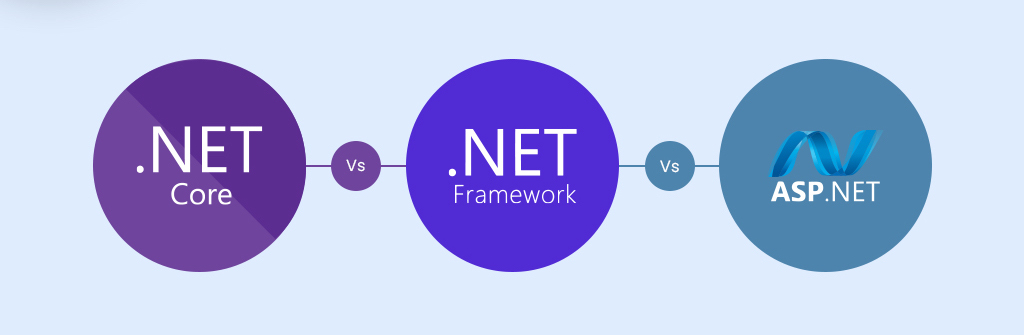
\includegraphics[width=1\textwidth]{Images/net vs.jpg}
\caption{\label{fig:net vs}Principali tecnologie Microsoft \gls{.net}.}
\end{figure}

Concludendo, \acrshort{asp.net} offre un \gls{framework} completo e versatile per lo sviluppo web. La sua architettura robusta, il supporto per lo sviluppo multi-piattaforma e l'integrazione con potenti strumenti di sviluppo lo rendono una scelta convincente per gli sviluppatori che mirano a fornire soluzioni web di alta qualità, scalabili e sicure.


\subsection{Swagger}\label{subsec:swagger}
\begin{figure}[H]
\centering

\includegraphics[width=0.4\textwidth]{Images/Swagger-logo.png}
\caption{\label{fig:swaggerlogo}Logo di Swagger.}
\end{figure}

Swagger è un insieme di strumenti per sviluppatori di \acrshort{api}, originariamente specificato e sviluppato da SmartBear Software. \cite{swagger}
È stato usato per testare il corretto funzionamento del back-end. Il suo vantaggio principale sta nella possibilità di essere utilizzato direttamente dal browser \cite{swagger.io}, senza dover installare alcun software aggiuntivo: è sufficiente digitare un indirizzo \acrshort{url} apposito e si aprirà una pagina web con un'interfaccia grafica dedicata, in cui ci sarà una lista di tutte le \acrshort{api} disponibili, sviluppate con \acrshort{asp.net} come si può vedere in figura \ref{fig:swagger}.
\begin{figure}[H]
\centering
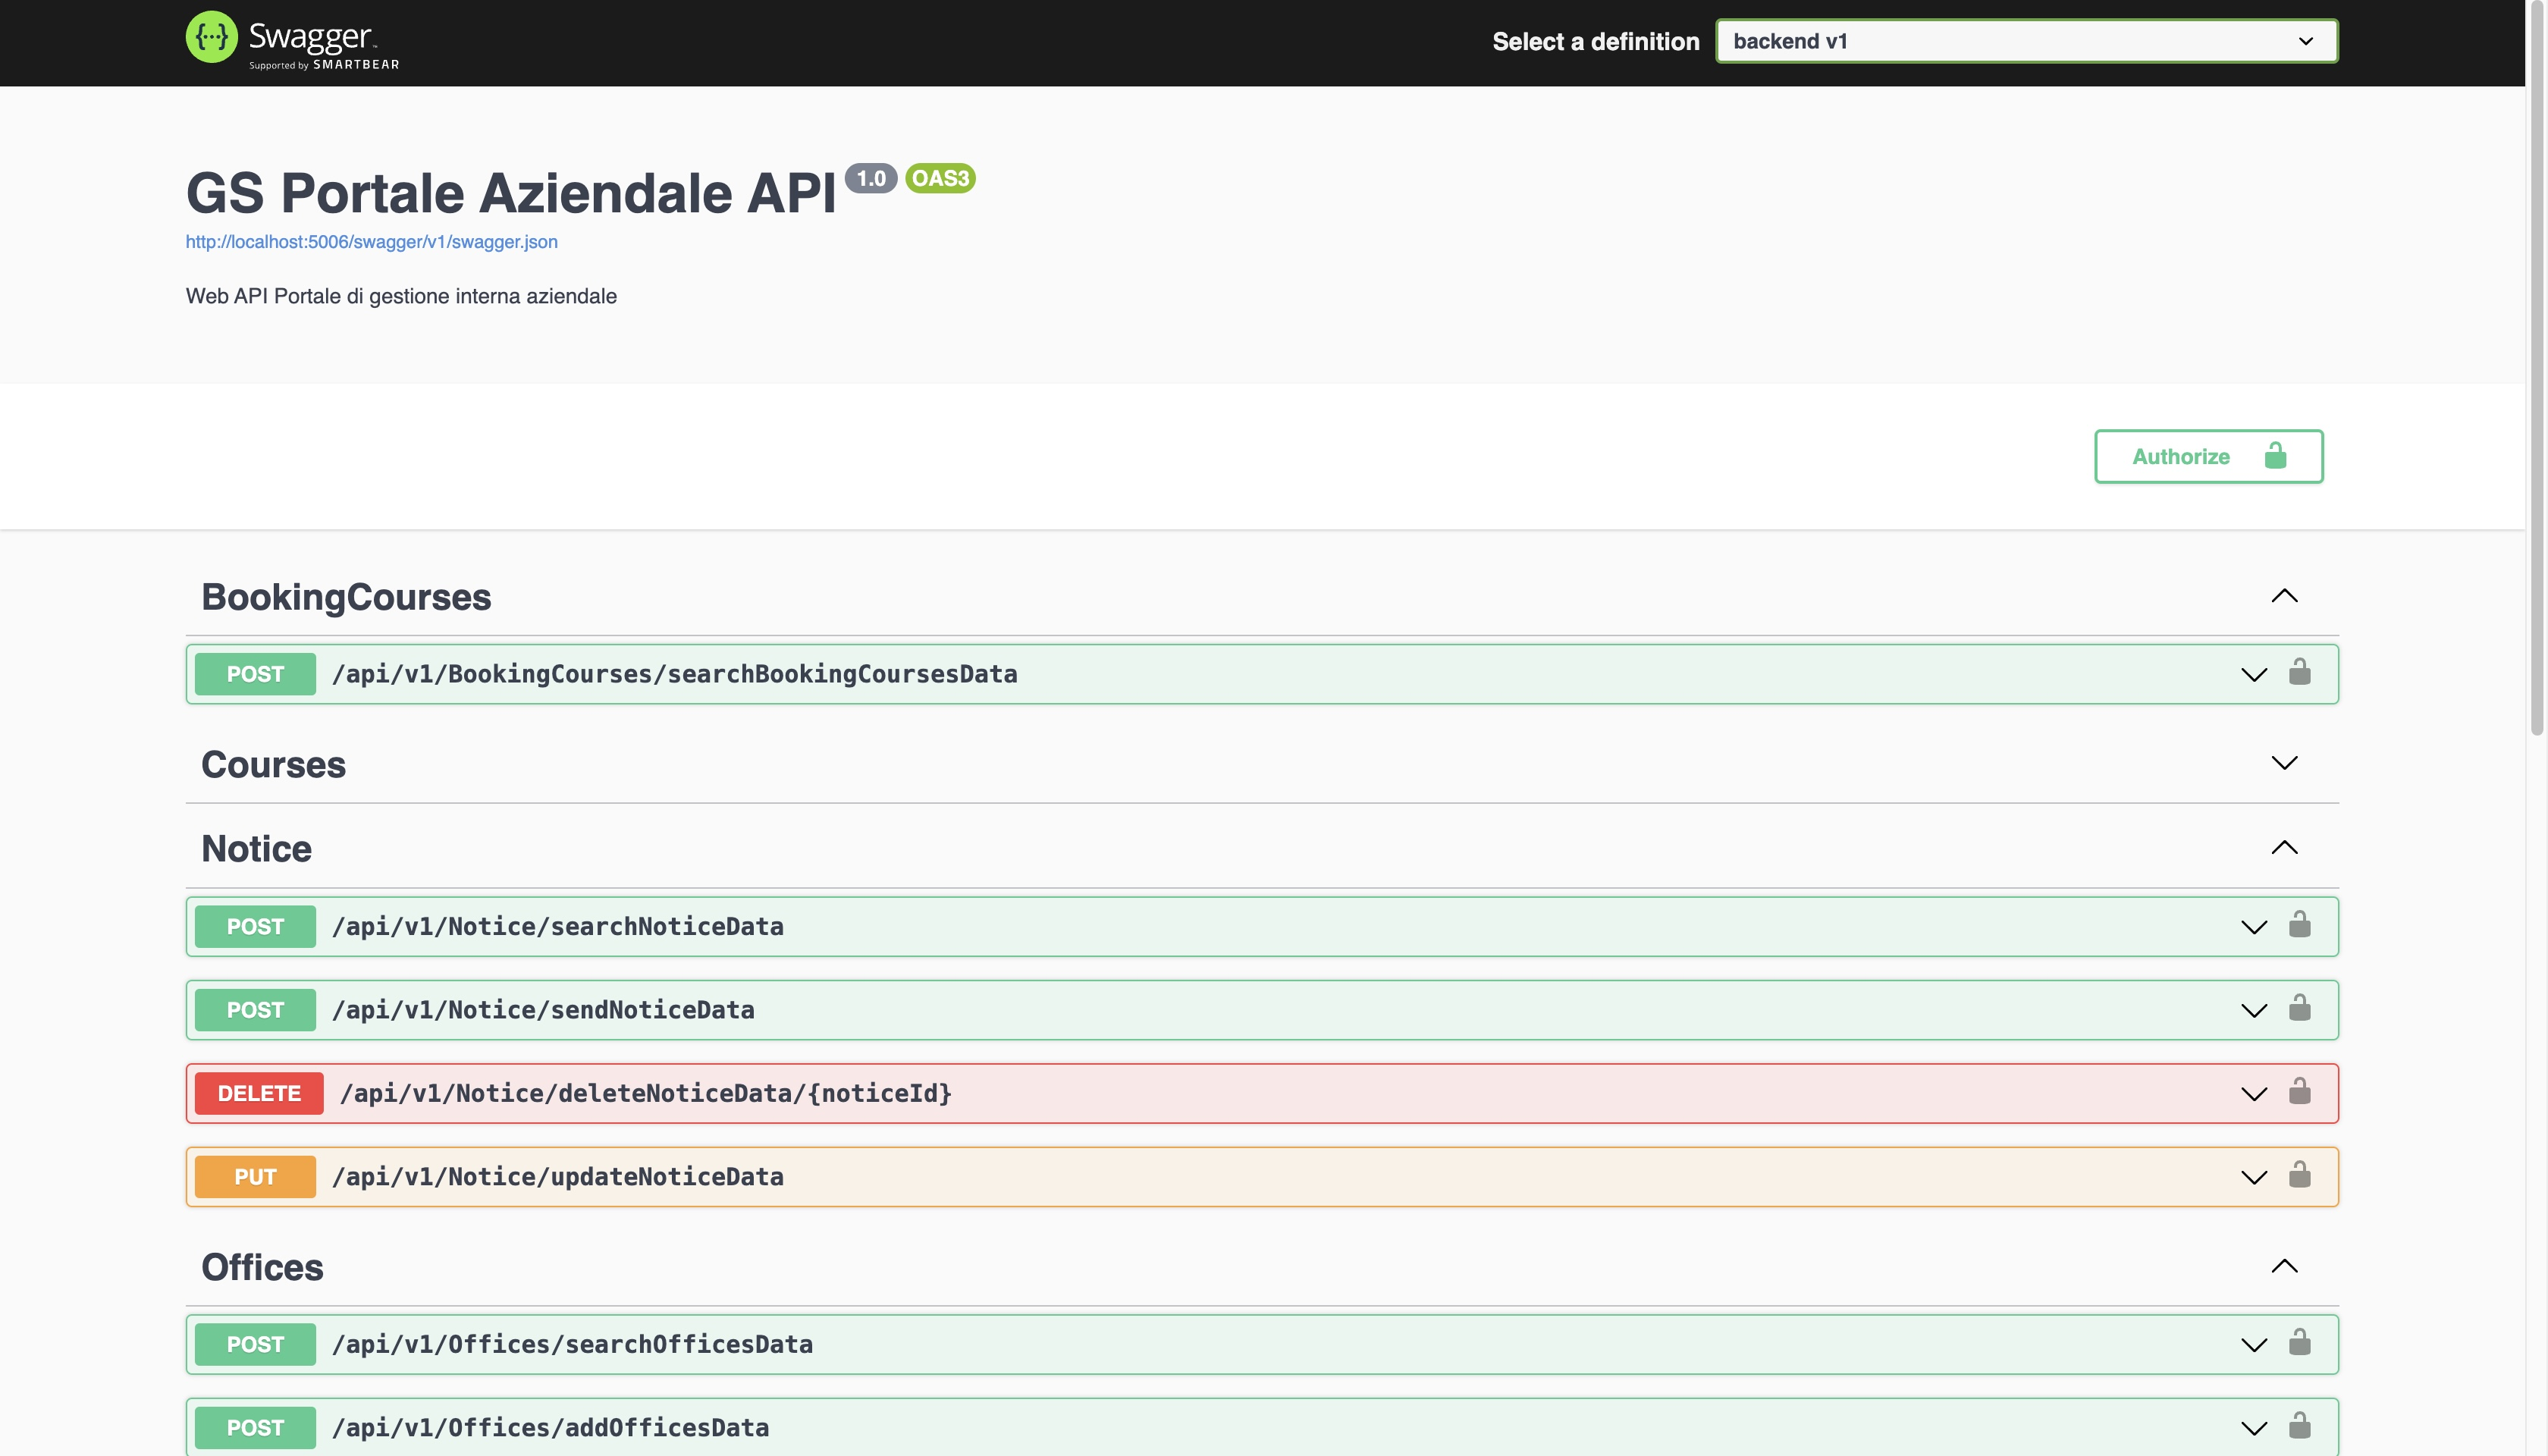
\includegraphics[width=1\textwidth]{Images/swagger.jpg}
\caption{\label{fig:swagger}Interfaccia grafica di Swagger, relativa al progetto di tirocinio.}
\end{figure}